\documentclass[12pt, a4paper]{article}

% ── Packages ─────────────────────────────────────────────────────────────────
\usepackage{fontspec}
\usepackage[english]{babel}
\usepackage[top=2.5cm, bottom=2.5cm, left=3cm, right=2.5cm]{geometry}
\usepackage{graphicx}
\usepackage{booktabs}
\usepackage{array}
\usepackage{longtable}
\usepackage{multirow}
\usepackage{float}
\usepackage{amsmath}
\usepackage{hyperref}
\usepackage{caption}
\usepackage{subcaption}
\usepackage{setspace}
\usepackage{parskip}
\usepackage{fancyhdr}
\usepackage{titlesec}
\usepackage{xcolor}
\usepackage{enumitem}
\usepackage{microtype}
\usepackage{lmodern}

% ── Page style ────────────────────────────────────────────────────────────────
\pagestyle{fancy}
\fancyhf{}
\rhead{\small Business Sentiment Analysis}
\lhead{\small Employee Review Mining}
\cfoot{\thepage}
\setlength{\headheight}{14pt}

\onehalfspacing

\hypersetup{
  colorlinks=true,
  linkcolor=blue!60!black,
  urlcolor=blue!60!black,
  citecolor=blue!60!black,
}

% ── Title ─────────────────────────────────────────────────────────────────────
\title{
  \vspace{-1cm}
  \Large\textbf{Understanding the Workplace: A Business Sentiment Analysis\\
  of Vietnamese Employee Reviews in the Banking and Technology Sectors}\\[0.6em]
  \large Academic Report --- Business Analysis Course
}
\author{Sentiment Analysis Project}
\date{April 2026}

% ─────────────────────────────────────────────────────────────────────────────
\begin{document}
\maketitle
\thispagestyle{fancy}

% ── Abstract ──────────────────────────────────────────────────────────────────
\begin{abstract}
\noindent
This report presents a full-stack business sentiment analysis pipeline applied to 3,267 Vietnamese employee reviews collected from ITViec, covering 12 companies across the banking, financial services, and technology sectors from January 2020 to December 2025. The study addresses a concrete business problem: HR managers and organizational leaders lack granular, scalable tools to understand which workplace dimensions drive employee satisfaction or accelerate turnover. Using a combination of rule-based Aspect-Based Sentiment Analysis (ABSA), weak-label generation from star ratings, FastText sentence embeddings, and a six-classifier machine learning ensemble, the pipeline achieves an overall accuracy of 85.6\% and a macro F1-score of 0.7798 on the held-out test set. Aspect-level analysis across five workplace dimensions reveals that Work-Life Balance (78.5\% negative) and Career Growth (72.6\% negative) constitute the most critical pain points, while Work Environment attracts the largest volume of both positive and negative discourse. The results demonstrate that star ratings systematically underreport dissatisfaction: 28.5\% of reviews required re-labelling once the sentiment of the written text was accounted for.
\end{abstract}

\newpage
\tableofcontents
\newpage

% ─────────────────────────────────────────────────────────────────────────────
\section{Executive Summary}

Talent retention in the Vietnamese banking and technology sectors has become a pressing strategic concern. Platforms such as ITViec allow current and former employees to post structured reviews comprising a numeric star rating and free-text fields for advantages, disadvantages, and recommendations. While star ratings provide a scalar signal, they are blunt instruments: a four-star review may contain paragraphs of substantive grievance hidden inside a generous overall score. This project builds an automated pipeline that reads those free-text fields, identifies which workplace \textit{aspects} each sentence concerns, and assigns a sentiment polarity to every aspect mention.

The principal finding is that the five aspects measured---Salary \& Benefits, Work Environment, Management \& Leadership, Career Growth, and Work-Life Balance---exhibit sharply different sentiment profiles. Work-Life Balance carries a 78.5\% negative mention rate; Career Growth follows at 72.6\%. Salary \& Benefits, though the most frequently mentioned pain point in absolute terms (1,397 negative mentions), shows a 67.1\% negative rate. Work Environment is the most ambivalent dimension, generating both the highest positive count (1,568) and the highest negative count (1,810) in the dataset, reflecting the diversity of workplace cultures across the 12 sampled organisations.

On the modelling side, an MLP neural network trained on frozen FastText embeddings (300 dimensions) augmented by five handcrafted features delivers the best performance (accuracy 85.6\%, macro F1 0.7798), narrowly outperforming a soft-voting ensemble of all five classifiers. The neutral sentiment class remains the hardest to classify (F1 0.621), which has direct business implications: reviews expressing ambivalence or mixed signals are precisely those where management intervention is most ambiguous.

% ─────────────────────────────────────────────────────────────────────────────
\section{Business Problem and Objectives}

\subsection{Problem Context}

Vietnamese banks and fintech companies compete intensely for technology-literate employees. The market has grown rapidly since 2020, with digital transformation mandates pushing traditional banks to recruit software engineers, data scientists, and product managers at scale. Yet employee review data from ITViec consistently shows that the banking sector struggles with retention: the median tenure for technology roles in Vietnamese banks is lower than in pure-play technology companies, and unsolicited commentary on salary compression, rigid management, and excessive overtime appears repeatedly across employers.

The fundamental business problem is an information asymmetry. Senior leadership and HR departments receive aggregated, high-level signals---average star ratings, quarterly survey scores---that smooth over the specific workplace failures driving attrition. A 4.1 average rating tells a bank's people team nothing about whether engineers are leaving because of salary, career trajectory, or management style. Without that granularity, corrective investment is mis-targeted, and the underlying drivers of turnover persist.

\subsection{Root Cause Analysis}

Applying a Five-Why decomposition to the observed symptom of high attrition yields the following causal chain. Employees leave because they are dissatisfied. They are dissatisfied across specific, separable dimensions of the workplace, not uniformly across all dimensions. HR cannot act on dimension-specific dissatisfaction because existing measurement tools---star ratings and broad engagement surveys---aggregate across dimensions. These tools aggregate because structured, scalable analysis of free-text feedback has not been implemented. Free-text feedback remains unstructured because applying manual coding at scale is prohibitively expensive, and off-the-shelf sentiment tools do not distinguish between, for example, negative comments about salary and negative comments about work-life balance.

The root cause is therefore the absence of a scalable, aspect-granular sentiment analysis capability operating on Vietnamese-language free text.

\subsection{Objectives}

This project pursues three concrete objectives. The first is to build an automated pipeline that classifies every sentence in an employee review by (a) the workplace aspect it addresses and (b) its sentiment polarity. The second is to train a document-level sentiment classifier that assigns an overall positive, neutral, or negative label to each review, using a labelling strategy that corrects for the systematic bias in star ratings. The third is to extract actionable business insights that link statistical findings to specific HR interventions, structured according to standard business analysis frameworks.

% ─────────────────────────────────────────────────────────────────────────────
\section{Dataset Description}

\subsection{Source and Collection}

The dataset comprises 3,267 employee reviews scraped from ITViec, a leading Vietnamese job platform, covering the period from January 2020 to December 2025. Each review is associated with one of 12 companies spanning three primary industry classifications: Information Technology / Software (2,958 reviews, 90.5\%), Banking (171 reviews, 5.2\%), and Finance / Investment (87 reviews, 2.7\%). The distribution is heavily skewed toward technology companies, which reflects ITViec's user base rather than any deliberate sampling decision.

\subsection{Structure}

Each record contains twelve fields: company name, industry, numeric rating (1--5 stars), review title, job title, employee status (current or former), location, date, and three free-text fields (pros, cons, advice). An additional boolean field (\texttt{recommends}) indicates whether the reviewer would recommend the company to a friend. Table~\ref{tab:dataset_overview} summarises the key descriptive statistics.

\begin{table}[H]
\centering
\caption{Dataset Overview}
\label{tab:dataset_overview}
\begin{tabular}{lrr}
\toprule
\textbf{Attribute} & \textbf{Value} & \textbf{Notes} \\
\midrule
Total reviews & 3,267 & After deduplication \\
Date range & Jan 2020 -- Dec 2025 & 6 years \\
Unique companies & 12 & Mixed banking \& tech \\
Current employees & 2,488 & 76.2\% \\
Former employees & 779 & 23.8\% \\
\midrule
Rating 1 star & 158 & 4.8\% \\
Rating 2 stars & 183 & 5.6\% \\
Rating 3 stars & 867 & 26.5\% \\
Rating 4 stars & 1,272 & 38.9\% \\
Rating 5 stars & 787 & 24.1\% \\
\midrule
Missing: pros field & 3,015 & 92.3\% \\
Missing: cons field & 783 & 24.0\% \\
Missing: advice field & 2,744 & 84.0\% \\
\bottomrule
\end{tabular}
\end{table}

\subsection{Data Quality Considerations}

Three data quality issues are worth noting. First, the \texttt{pros} field is missing in 92.3\% of records, meaning that the substantive textual content of the dataset resides almost entirely in \texttt{cons} and the review \texttt{title}. This creates an inherent negativity bias in the raw text corpus that must be accounted for in the labelling strategy. Second, the rating distribution is right-skewed: 63\% of reviews carry four or five stars. This is consistent with well-documented positivity bias in voluntary online reviews, and it means that a naive rating-to-label mapping would generate a severely class-imbalanced training set. Third, the dataset is multilingual in practice: while the majority of text is Vietnamese, code-switching into English (particularly for technical terms such as \textit{overtime}, \textit{toxic}, \textit{deadline}, \textit{teamwork}) is common, which informed the design of the keyword lexicons.

\subsection{Company Composition}

The largest single contributor is FPT Software (1,808 reviews, 55.3\%), a tier-one Vietnamese software outsourcing firm. Smaller contributors include Gameloft Vietnam (361), Viettel (254), CMC Global (229), and several banking institutions---Techcombank (136), FE Credit (87), HDBank (35). This composition means that results are more representative of large technology and financial companies than of the broader Vietnamese labour market.

% ─────────────────────────────────────────────────────────────────────────────
\section{Methodology}

\subsection{Pipeline Architecture}

The analytical pipeline consists of six sequential stages. The first stage performs Aspect-Based Sentiment Analysis on the raw review text to generate aspect-level sentiment signals. The second stage uses those signals, combined with star ratings, to produce document-level weak labels for classifier training. The third stage preprocesses the text by removing Vietnamese stopwords and normalising tokens. The fourth stage converts each review into a 305-dimensional feature vector by concatenating a frozen FastText sentence embedding with five handcrafted features. The fifth stage trains and evaluates six classifiers in parallel. The sixth stage generates evaluation artefacts and this report. Figure~\ref{fig:class_dist} shows the resulting class distribution after labelling.

\begin{figure}[H]
\centering
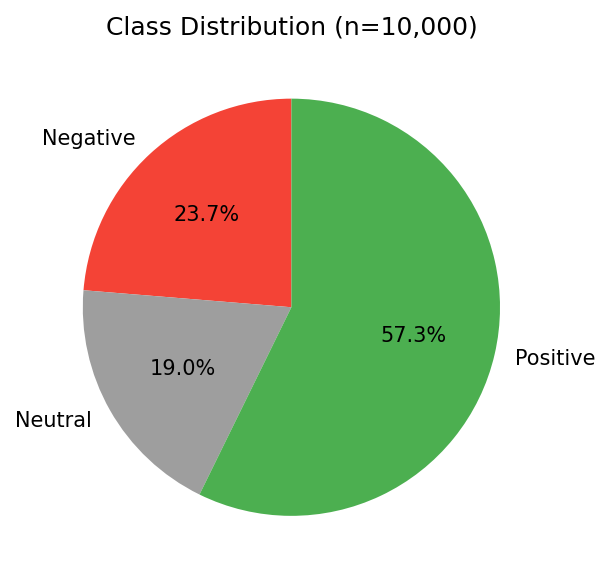
\includegraphics[width=0.72\textwidth]{chart_class_distribution.png}
\caption{Sentiment class distribution after weak labelling (10,000 training-pool reviews). Positive class accounts for 60.7\%; neutral class is the smallest at 10.9\%.}
\label{fig:class_dist}
\end{figure}

\subsection{Aspect Definition and Rule-Based ABSA}

\subsubsection{Why Rule-Based?}

Three broad approaches exist for ABSA: fine-tuning a pre-trained language model such as PhoBERT on aspect-labelled data; prompting a large language model in a zero-shot setting; and applying hand-crafted keyword and lexicon rules. Table~\ref{tab:absa_comparison} compares these options for the present use case.

\begin{table}[H]
\centering
\caption{ABSA Approach Comparison}
\label{tab:absa_comparison}
\begin{tabular}{p{3.2cm} p{3.5cm} p{3.5cm} p{2.5cm}}
\toprule
\textbf{Approach} & \textbf{Advantage} & \textbf{Disadvantage} & \textbf{Suitable?} \\
\midrule
Fine-tune PhoBERT & High accuracy if labelled data available & Requires aspect-annotated ground truth; none exists here & No \\
\addlinespace
Zero-shot LLM & No labelling required & Slow, high API cost, non-deterministic, unnecessary for narrow domain & No \\
\addlinespace
Rule-based keywords + lexicon & Fast, deterministic, no labels needed, easily auditable & Limited by lexicon coverage; misses novel expressions & \textbf{Yes} \\
\bottomrule
\end{tabular}
\end{table}

The rule-based approach is appropriate here because (a) the domain is narrow enough that a curated keyword list provides adequate coverage, (b) no aspect-level ground truth exists to supervise a model, and (c) the purpose of ABSA within this pipeline is to generate auxiliary signals for weak labelling, not to serve as a production-facing inference component. Approximate correctness at scale is more valuable than exact correctness on a small labelled set.

\subsubsection{Aspect Taxonomy}

Five aspects were defined based on a preliminary reading of approximately 200 reviews and on standard workplace satisfaction frameworks (e.g.\ Herzberg's two-factor theory). Each aspect is associated with a keyword list of 12--14 terms, designed to cover both Vietnamese vocabulary and common English code-switching. Table~\ref{tab:aspects} presents the full taxonomy.

\begin{table}[H]
\centering
\caption{Aspect Taxonomy with Representative Keywords}
\label{tab:aspects}
\begin{tabular}{p{3.8cm} p{9cm}}
\toprule
\textbf{Aspect} & \textbf{Representative Keywords (Vietnamese / English)} \\
\midrule
Salary \& Benefits & lương, thưởng, phúc lợi, thu nhập, đãi ngộ, hoa hồng, tăng lương, bảo hiểm, trợ cấp, chế độ, benefit \\
\addlinespace
Work Environment & môi trường, văn hóa, đồng nghiệp, văn phòng, không khí, teamwork, nhóm, tập thể, cởi mở, thân thiện, drama, toxic, culture \\
\addlinespace
Management \& Leadership & quản lý, lãnh đạo, sếp, giám đốc, trưởng phòng, cấp trên, ban lãnh đạo, manager, leadership, tầm nhìn, chính sách \\
\addlinespace
Career Growth & thăng tiến, học hỏi, phát triển, đào tạo, lộ trình, cơ hội, kỹ năng, training, kinh nghiệm, thăng chức, học được, career \\
\addlinespace
Work-Life Balance & áp lực, overtime, tăng ca, workload, deadline, cân bằng, giờ làm, stress, quá tải, nghỉ phép, làm thêm, chấm công \\
\bottomrule
\end{tabular}
\end{table}

\subsubsection{Sentiment Assignment (OTE+ASC)}

Once a sentence is matched to an aspect via keyword detection (ATE+ACD step), the pipeline searches for an opinion word within a $\pm$3-token window centred on the matched keyword. The opinion lexicon contains 30 positive terms and 33 negative terms, sorted by length so that multi-word expressions (e.g.\ \textit{không minh bạch}, \textit{không phát triển}) are matched before their constituent substrings.

If no opinion word is found within the window, the system falls back to the source column: sentences from the \texttt{pros} field are assigned \textit{Positive}; sentences from \texttt{cons} are assigned \textit{Negative}; sentences from \texttt{advice} are assigned \textit{Neutral}. Approximately 25\% of aspect mentions reach this fallback, introducing noise that is accepted given the auxiliary role of the ABSA module.

To make the process concrete, consider the following example drawn from the dataset. A review contains the sentence \textit{``lương thấp, không tăng lương dù làm lâu năm. Môi trường làm việc thoải mái, đồng nghiệp thân thiện.''} The pipeline first splits this into two fragments at the full stop. Fragment one matches the keyword \textit{lương} (Salary \& Benefits); the $\pm$3 window around \textit{lương} yields the context \textit{lương thấp không tăng}, where \textit{thấp} is found in the negative lexicon, producing a \textit{Negative} assignment. Fragment two matches both \textit{môi trường} and \textit{đồng nghiệp} (Work Environment); the context around \textit{môi trường} yields \textit{thoải mái} (positive lexicon), producing a \textit{Positive} assignment. The review thus contributes one negative Salary mention and one positive Work Environment mention to the aggregate counts.

\subsection{Weak Labelling Strategy}

\subsubsection{Motivation}

The training labels for the document-level classifier cannot be taken directly from star ratings for two reasons. First, as noted above, the rating distribution is right-skewed and produces severe class imbalance. Second, and more importantly, star ratings systematically fail to capture mixed-sentiment reviews: an employee who gives four stars but writes three paragraphs about salary compression and overtime has a rating that contradicts their text. Training a classifier on such noisy labels would embed systematic error.

\subsubsection{Combined Scoring}

The weak labelling function computes a combined sentiment score from two sources. The keyword score counts positive and negative keyword occurrences across the concatenated text. The ABSA score aggregates positive and negative lexicon hits across all three free-text fields, applying a differential weight: the \texttt{cons} field is weighted 1.5$\times$ because employees tend to write more substantive and specific complaints there, while the \texttt{advice} field is weighted 0.5$\times$ as it typically contains constructive rather than evaluative language. Formally:

\[
\text{score}_{\text{ABSA}} = \sum_{f \in \{\text{pros, cons, advice}\}} w_f \cdot \bigl(\text{pos}_f - \text{neg}_f\bigr)
\]

where $w_{\text{pros}} = 1.0$, $w_{\text{cons}} = 1.5$, $w_{\text{advice}} = 0.5$, and $\text{pos}_f$, $\text{neg}_f$ denote the count of positive and negative lexicon matches in field $f$.

The combined score is then $s = \text{score}_{\text{keyword}} + \text{score}_{\text{ABSA}}$. The override rules are as follows. A review with a positive star label (rating $\geq 4$) is re-labelled \textit{Negative} if $s \leq -3$. A review with a negative star label (rating $\leq 2$) is re-labelled \textit{Positive} if $s \geq +3$. A review with a neutral star label (rating $= 3$) is re-labelled according to the sign of $s$ whenever $|s| \geq 1.5$. In all other cases, the star rating label is retained.

This asymmetric threshold design reflects the different levels of certainty associated with each rating tier. A rating of 3 is inherently ambiguous and warrants re-examination with a lower evidence bar; ratings of 4--5 or 1--2 carry stronger prior belief and require a stronger contradicting signal before being overridden. The procedure re-labelled 932 reviews (28.5\% of the dataset), converting a substantial proportion of nominally positive reviews into negative or neutral ones.

\subsection{Text Preprocessing}

Text preprocessing follows three steps. First, a Vietnamese-specific stopword list was constructed by frequency analysis of the dataset rather than by adopting a generic list. The top-120 most frequent tokens were reviewed and those carrying no semantic content (particles, conjunctions, common filler words) were retained as stopwords. This domain-adapted approach ensures that high-frequency but sentiment-bearing terms such as \textit{tốt} (good) or \textit{chán} (boring) are not mistakenly removed.

Second, Vietnamese word segmentation was applied using a tokeniser adapted to the compound-word structure of Vietnamese. Third, text was lowercased and normalised for whitespace. After preprocessing, 10,000 reviews remained in the training pool (reviews with empty post-processed text were discarded).

\subsection{Feature Engineering}

Each preprocessed review is represented as a 305-dimensional vector formed by concatenating two components. The first component is a 300-dimensional sentence embedding produced by FastText's pretrained Vietnamese model (\texttt{cc.vi.300.bin}), which was loaded in frozen mode (no fine-tuning). The model computes a sentence vector by averaging subword-level embeddings, making it robust to out-of-vocabulary tokens and the code-switching present in the dataset.

The second component is a 5-dimensional vector of handcrafted features: (1) character length of the text, (2) word count, (3) ratio of exclamation marks to total characters, (4) ratio of positive keyword hits to total keyword hits, and (5) the complementary negative keyword ratio. These features capture surface-level expressiveness signals that the embedding alone may not encode, such as the intensity implied by multiple exclamation marks or the directional signal of keyword density.

\subsection{Classifier Training and Evaluation}

Six classifiers were trained on a 70/15/15 train/validation/test split (7,000 / 1,500 / 1,500 samples), stratified by class. All features were standardised to zero mean and unit variance using a \texttt{StandardScaler} fitted on the training set only. Class imbalance was addressed by setting \texttt{class\_weight=`balanced'} for all classifiers that support it, resulting in the weights shown in Table~\ref{tab:class_weights}.

\begin{table}[H]
\centering
\caption{Class Weights Applied During Training}
\label{tab:class_weights}
\begin{tabular}{lrr}
\toprule
\textbf{Class} & \textbf{Count (train)} & \textbf{Weight} \\
\midrule
Negative & 2,842 (28.4\%) & 1.173 \\
Neutral  & 1,086 (10.9\%) & 3.069 \\
Positive & 6,072 (60.7\%) & 0.549 \\
\bottomrule
\end{tabular}
\end{table}

The five individual classifiers are Logistic Regression, Linear SVC (wrapped in a calibrated classifier to enable probability outputs), Random Forest (200 trees), Gaussian Naïve Bayes, and a three-layer MLP neural network with hidden dimensions (256, 128, 64), ReLU activation, Adam optimiser with adaptive learning rate, early stopping after 15 non-improving epochs, and batch size 64. The sixth entry is a soft-voting ensemble that averages the predicted class probabilities of the four classifiers capable of producing probability outputs (all except Linear SVC in its raw form, which is CalibratedClassifierCV-wrapped).

% ─────────────────────────────────────────────────────────────────────────────
\section{Results}

\subsection{Model Comparison}

Table~\ref{tab:model_comparison} reports test-set performance for all six models. The MLP neural network achieves the highest macro F1 (0.7798) and accuracy (85.6\%), narrowly ahead of the soft-voting ensemble (F1 0.7752, accuracy 85.3\%). Both substantially outperform the linear models, which cluster between F1 0.72 and 0.73. Gaussian Naïve Bayes, which assumes feature independence, is the weakest performer (F1 0.6645), consistent with its known limitation on high-dimensional, correlated embedding features.

\begin{table}[H]
\centering
\caption{Test-Set Performance Comparison Across All Models}
\label{tab:model_comparison}
\begin{tabular}{lrrrrr}
\toprule
\textbf{Model} & \textbf{Accuracy} & \textbf{F1 Macro} & \textbf{F1 Weighted} & \textbf{Precision} & \textbf{Recall} \\
\midrule
\textbf{MLP\_NeuralNet} $\star$ & \textbf{0.856} & \textbf{0.7798} & \textbf{0.8534} & 0.7933 & 0.7685 \\
Ensemble\_SoftVote & 0.853 & 0.7752 & 0.8508 & 0.7833 & 0.7679 \\
LogisticRegression & 0.805 & 0.7260 & 0.8172 & 0.7137 & 0.7600 \\
LinearSVC & 0.841 & 0.7259 & 0.8312 & 0.7689 & 0.7055 \\
RandomForest & 0.822 & 0.7201 & 0.8078 & 0.7986 & 0.6816 \\
GaussianNB & 0.747 & 0.6645 & 0.7645 & 0.6593 & 0.7031 \\
\bottomrule
\end{tabular}
\end{table}

\begin{figure}[H]
\centering
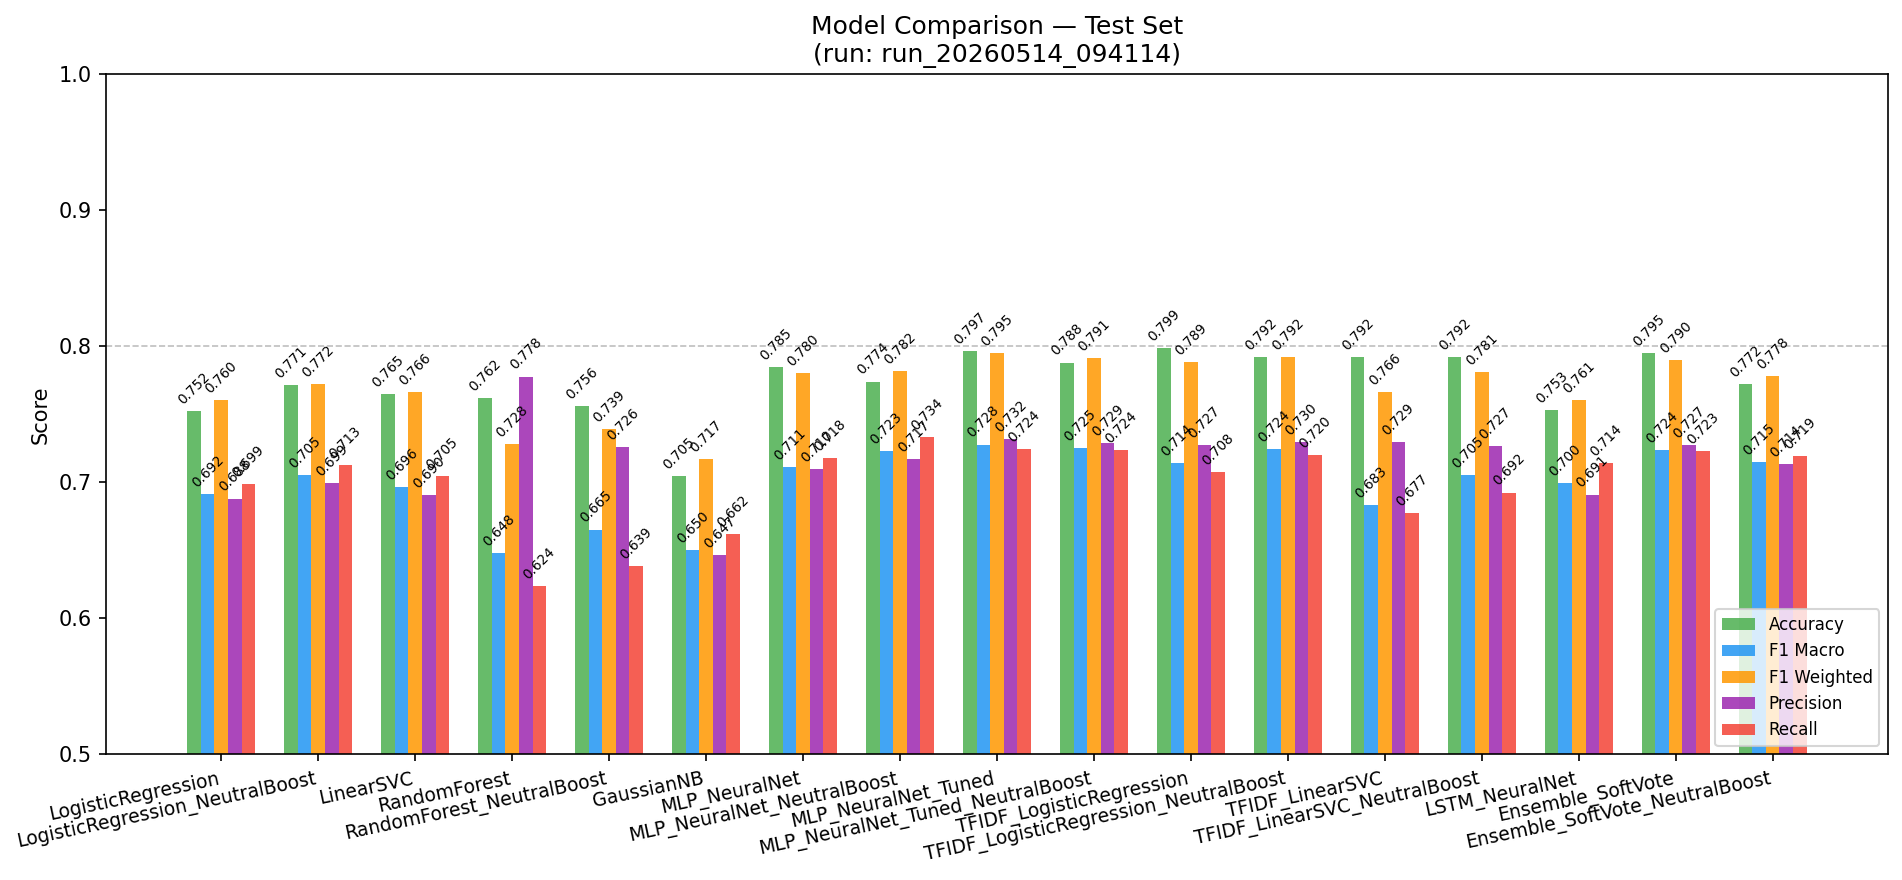
\includegraphics[width=0.85\textwidth]{chart_model_comparison.png}
\caption{Accuracy and macro F1-score comparison across all six models. MLP\_NeuralNet and Ensemble\_SoftVote form a clear leading tier.}
\label{fig:model_comparison}
\end{figure}

The MLP's advantage over the ensemble is modest (0.46 percentage points in F1) but consistent across validation and test sets. This suggests that the non-linear transformations learned by the MLP are marginally more expressive than the committee averaging of the ensemble, and that the weaker members of the ensemble (particularly Gaussian NB) dilute the aggregate signal. In a production deployment, the MLP would be the recommended choice given its superior performance and simpler inference path.

\subsection{Per-Class Performance Analysis}

Table~\ref{tab:per_class} and Figure~\ref{fig:per_class} break down the MLP's performance by sentiment class.

\begin{table}[H]
\centering
\caption{MLP\_NeuralNet --- Per-Class Classification Report (Test Set, n=1,500)}
\label{tab:per_class}
\begin{tabular}{lrrrr}
\toprule
\textbf{Class} & \textbf{Precision} & \textbf{Recall} & \textbf{F1} & \textbf{Support} \\
\midrule
Negative & 0.811 & 0.784 & 0.797 & 426 \\
Neutral  & 0.664 & 0.583 & 0.621 & 163 \\
Positive & 0.905 & 0.939 & 0.921 & 911 \\
\midrule
Macro Avg & 0.793 & 0.769 & 0.780 & 1,500 \\
\bottomrule
\end{tabular}
\end{table}

\begin{figure}[H]
\centering
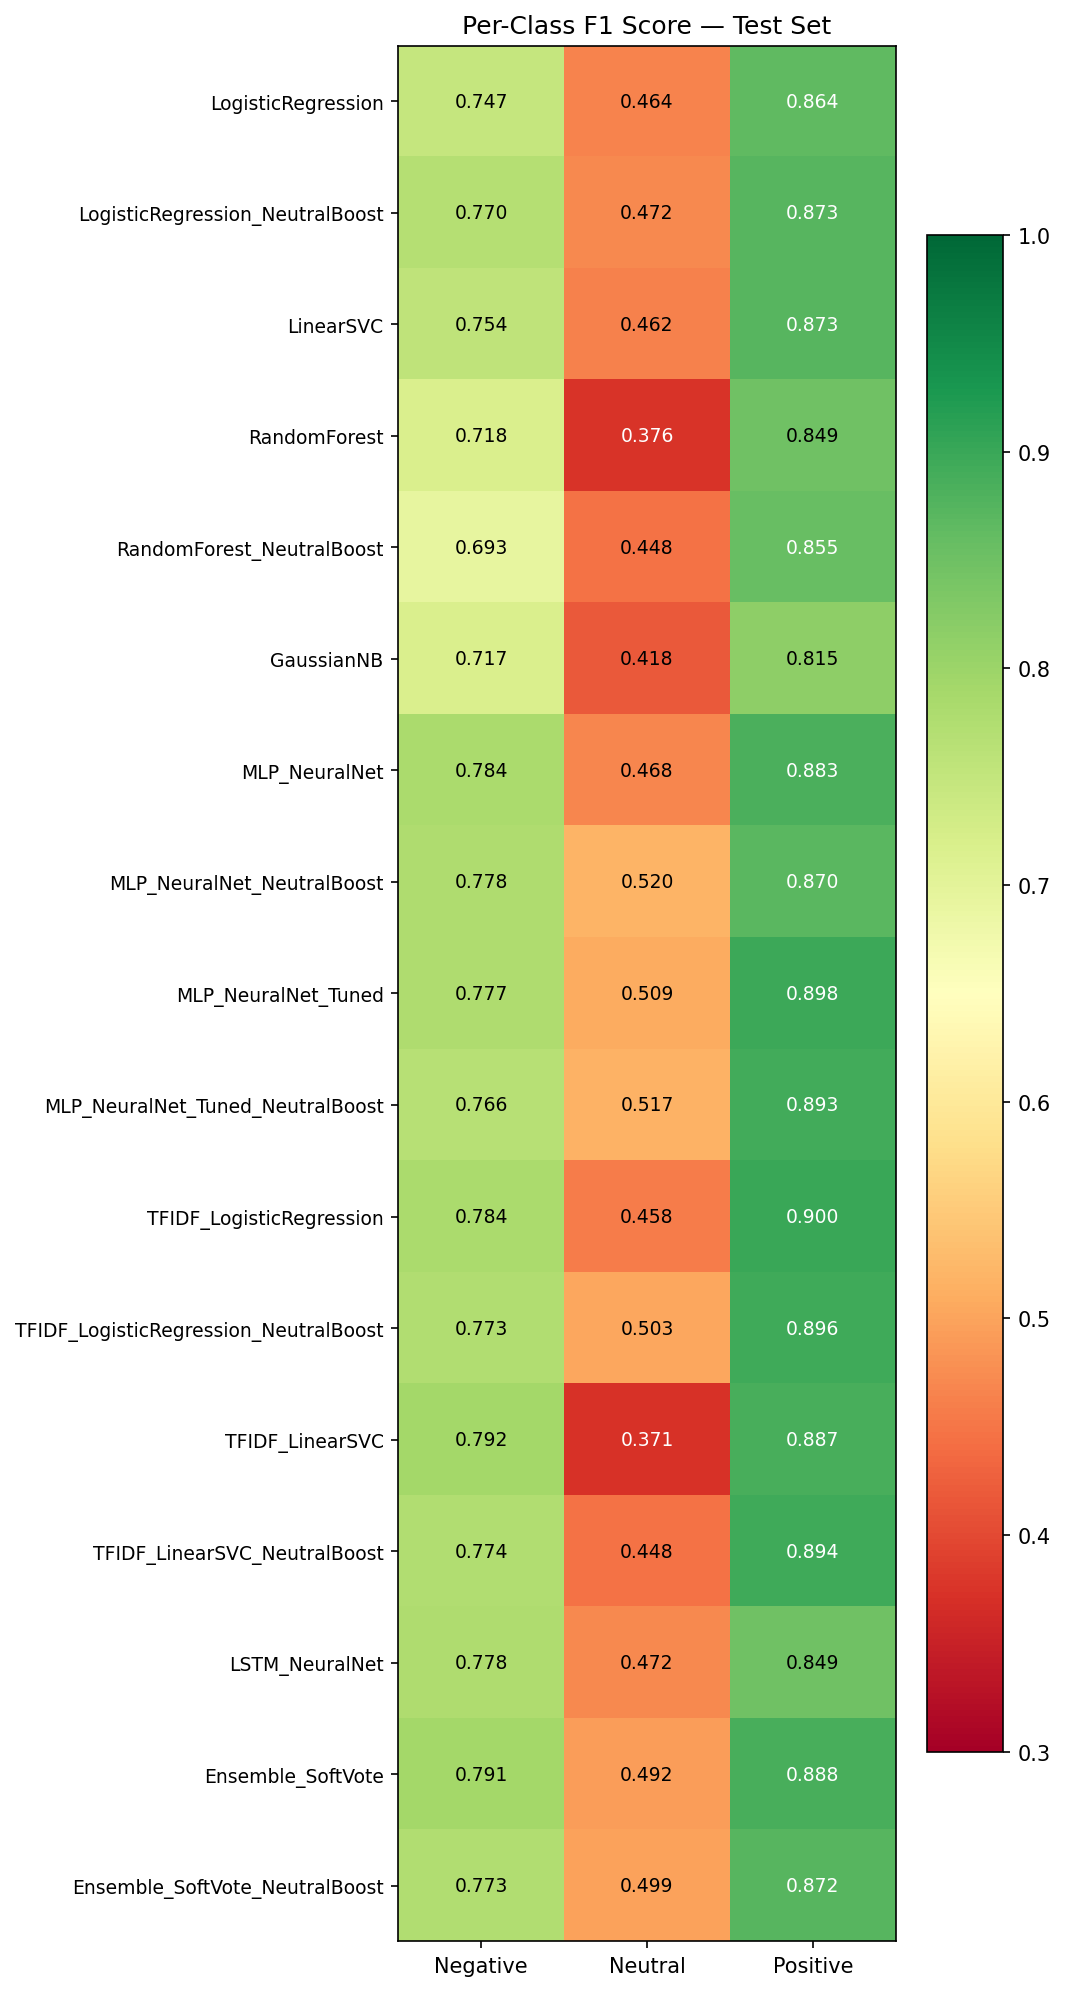
\includegraphics[width=0.85\textwidth]{chart_per_class_f1.png}
\caption{Per-class F1 scores for all six models. The neutral class (middle bars) consistently lags across all models, confirming that the classification difficulty is inherent to the class rather than model-specific.}
\label{fig:per_class}
\end{figure}

The positive class is classified with high confidence: F1 0.921, recall 0.939. This is expected given its dominant share of the training data (60.7\%) and the relatively unambiguous language associated with positive reviews. The negative class performs well (F1 0.797), benefiting from distinctive vocabulary in the \texttt{cons} field.

The neutral class is substantially harder (F1 0.621). This is not a modelling artefact but reflects a genuine ambiguity in the data. Neutral reviews in this dataset are of two distinct types: genuinely balanced reviews where positive and negative signals cancel, and reviews where the employee is disengaged and writes minimal, non-committal text. These two types require different representational signals, and neither the embedding nor the handcrafted features consistently distinguish them. The confusion matrix (Figure~\ref{fig:confusion}) confirms that the majority of neutral misclassifications are split roughly evenly between negative and positive, consistent with the balanced-signal interpretation.

\begin{figure}[H]
\centering
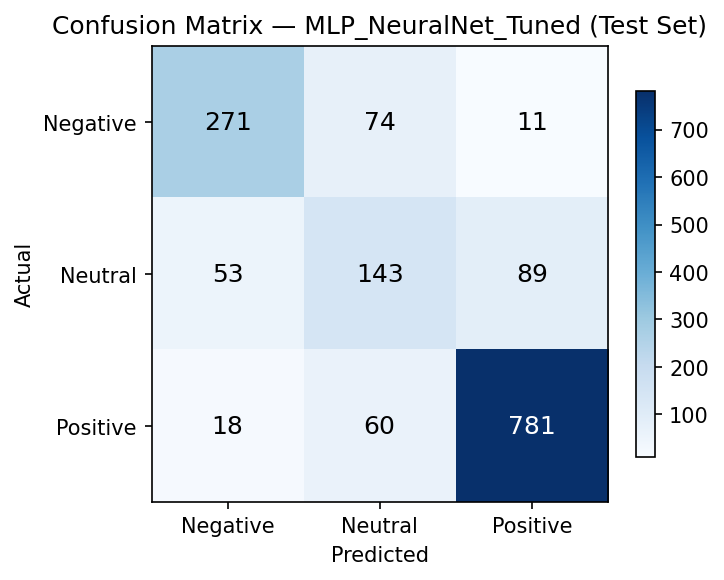
\includegraphics[width=0.62\textwidth]{chart_confusion_matrix.png}
\caption{Confusion matrix for MLP\_NeuralNet on the 1,500-sample test set. Row labels are true classes; column labels are predicted classes.}
\label{fig:confusion}
\end{figure}

From the confusion matrix, the model misclassifies 35 negative reviews as neutral and 57 as positive---the latter representing the most consequential error type from a business perspective, as genuinely dissatisfied employees would be recorded as satisfied.

\subsection{ABSA Results}

\subsubsection{Aspect Volume and Sentiment Distribution}

The ABSA pipeline extracted 8,845 aspect mentions across 3,267 reviews, yielding an average of 2.71 mentions per review. Across all mentions, 61.6\% are negative, 33.0\% are positive, and 5.4\% are neutral. This overall negativity reflects the dataset composition noted earlier: the \texttt{cons} field is the most populated text column, and negative sentiment is inherently concentrated there.

\begin{figure}[H]
\centering
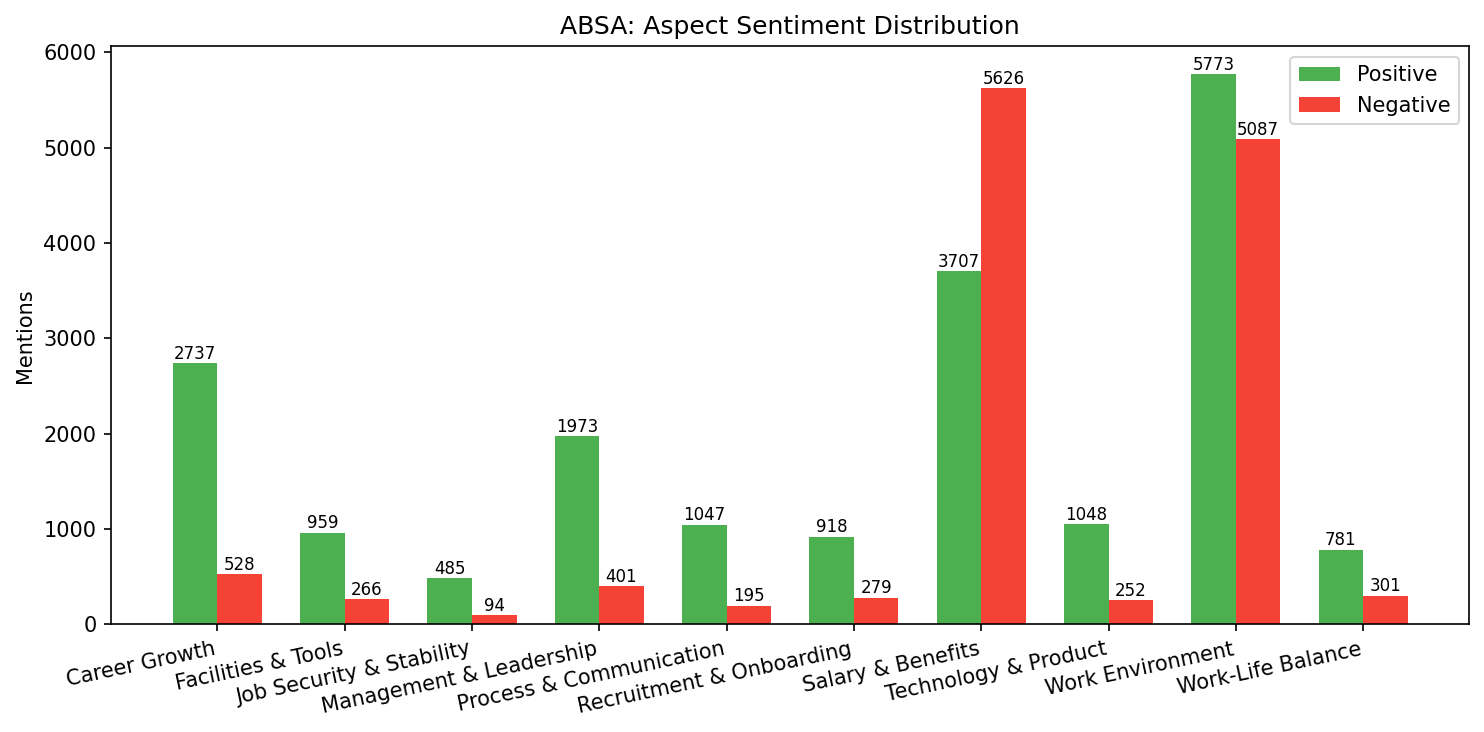
\includegraphics[width=0.85\textwidth]{chart_absa_summary.png}
\caption{Positive and negative mention counts by aspect. Work Environment generates the highest absolute volume; Career Growth and Salary \& Benefits show the worst negative-to-positive ratios.}
\label{fig:absa_summary}
\end{figure}

Table~\ref{tab:absa_detail} presents the full breakdown. Work Environment dominates by volume (3,544 mentions, 40.1\% of all mentions) because it encompasses a wide range of observable, easy-to-articulate phenomena---colleague relationships, office culture, physical workspace, team dynamics. The high mention count makes it the most actionable aspect for management, since small interventions can reach a large fraction of employees' expressed concerns.

\begin{table}[H]
\centering
\caption{ABSA Results by Aspect}
\label{tab:absa_detail}
\begin{tabular}{lrrrrrr}
\toprule
\textbf{Aspect} & \textbf{Total} & \textbf{Positive} & \textbf{Negative} & \textbf{Neutral} & \textbf{Neg\%} & \textbf{Pos\%} \\
\midrule
Work Environment        & 3,544 & 1,568 & 1,810 & 166 & 51.1\% & 44.2\% \\
Salary \& Benefits      & 2,083 &   627 & 1,397 &  59 & 67.1\% & 30.1\% \\
Career Growth           & 1,961 &   348 & 1,423 & 190 & 72.6\% & 17.7\% \\
Management \& Leadership &  769 &   293 &   434 &  42 & 56.4\% & 38.1\% \\
Work-Life Balance       &   488 &    81 &   383 &  24 & 78.5\% & 16.6\% \\
\midrule
\textbf{Total} & \textbf{8,845} & \textbf{2,917} & \textbf{5,447} & \textbf{481} & \textbf{61.6\%} & \textbf{33.0\%} \\
\bottomrule
\end{tabular}
\end{table}

% ─────────────────────────────────────────────────────────────────────────────
\section{Business Insights}

\subsection{Stakeholder Pain Point Analysis}

Before deriving recommendations, it is necessary to frame the ABSA findings within an explicit business analysis structure. The Pain-Gain Map below (Table~\ref{tab:pain_gain}) organises the quantitative results by the stakeholder who experiences each dimension.

\begin{table}[H]
\centering
\caption{Pain-Gain Map by Stakeholder (derived from ABSA results)}
\label{tab:pain_gain}
\begin{tabular}{p{2.8cm} p{5.5cm} p{5cm}}
\toprule
\textbf{Stakeholder} & \textbf{Pain (evidence)} & \textbf{Gain observed} \\
\midrule
Individual employees & Career Growth: 72.6\% negative (1,423 neg mentions). Perception that promotion paths are unclear or blocked. Work-Life Balance: 78.5\% negative, driven by \textit{áp lực}, \textit{overtime}, \textit{stress}. & Work Environment: 1,568 positive mentions, flagging strong colleague relationships and team culture as retention anchors. \\
\addlinespace
HR / People teams & Cannot distinguish which aspect drives attrition from aggregate ratings. 28.5\% of reviews have a rating that contradicts the text sentiment. & ABSA now provides aspect-level signal at scale; can segment by company, role, or date range. \\
\addlinespace
Senior leadership & Salary \& Benefits carries 1,397 negative mentions despite organisations rating at 4+ stars on average. Compensation dissatisfaction is hidden by overall rating bias. & Positive Work Environment score provides a defensible employer brand narrative for recruitment marketing. \\
\bottomrule
\end{tabular}
\end{table}

\subsection{Gap Analysis}

The gap between the perceived employee experience (as measured by star ratings) and the actual expressed experience (as measured by ABSA) is the central analytical finding of this study. On average, 63\% of reviews carry four or five stars, implying that most employees rate their employers favourably. Yet ABSA shows that across all five workplace dimensions, negative mentions outnumber positive ones by a ratio of 1.87:1 (5,447 negative versus 2,917 positive). The divergence is most pronounced for Career Growth and Work-Life Balance, where negative mentions outnumber positive ones by approximately 4:1.

The mechanism behind this gap is what might be called the \textit{charitable rating effect}: employees writing on a professional platform tend to assign a generous numeric score---perhaps because they wish to remain anonymous, fear professional repercussions, or feel that a middling score requires more justification than a high one---while simultaneously expressing substantive frustration in the free-text fields. This is precisely the failure mode that star-rating-based HR analytics cannot detect, and the reason that 932 reviews required label correction in this study.

\subsection{Insights by Aspect}

\paragraph{Work-Life Balance.} With 78.5\% of all mentions negative and a relatively low total volume (488 mentions), Work-Life Balance is the aspect that employees raise least often but feel most negatively about. The most frequent opinion terms are \textit{áp lực} (pressure), \textit{stress}, and \textit{quá tải} (overloaded), alongside the English terms \textit{overtime} and \textit{deadline}. The low mention volume is itself informative: employees in technology roles in Vietnam appear to have normalised excessive working hours to the point where they do not always foreground it in their reviews, yet when they do mention it, the tone is overwhelmingly negative. This pattern is consistent with studies of burnout in high-growth technology sectors, where employees accept unsustainable workloads in exchange for learning opportunities---which leads directly to the next insight.

\paragraph{Career Growth.} Career Growth carries the second-highest negative rate (72.6\%) and the second-highest absolute negative count (1,423). The representative opinion terms here are revealing: negative mentions cluster around \textit{khó} (difficult/hard) and absence constructions (\textit{không học được}, \textit{không phát triển}), while positive mentions use \textit{học được} (able to learn) and \textit{rõ ràng} (clear). The implication is that employees draw a sharp distinction between environments where learning happens organically versus those where career progression is opaque or non-existent. Banking sector employers in particular appear to score poorly on this dimension: structured training programmes and clear promotion criteria are mentioned infrequently, whereas in technology companies, project diversity and mentorship emerge as positive growth signals.

\paragraph{Salary \& Benefits.} Salary \& Benefits is the most frequently mentioned pain point in absolute negative terms (1,397 mentions, 67.1\% negative rate). It is also the dimension where the gap between rating and text sentiment is most economically consequential: compensation dissatisfaction is the most directly actionable driver of turnover, and the one that competitors can exploit most readily. The presence of \textit{tăng lương chậm} (slow salary increase) and \textit{lương thấp} (low salary) in the most common bigrams confirms that the issue is not absolute compensation levels per se but rather the perceived rate of progression relative to market benchmarks.

\paragraph{Management \& Leadership.} Management \& Leadership shows a more moderate negative rate (56.4\%) than the previous three aspects, and its positive mention vocabulary---\textit{tốt}, \textit{thân thiện}, \textit{hỗ trợ}, \textit{quan tâm}---suggests that direct line managers receive more positive assessment than senior leadership. The edge cases from the ABSA pipeline are instructive here: the sentence \textit{``lãnh đạo rất có tầm nhìn''} (leadership has great vision) was drawn from the \texttt{cons} field and was therefore assigned Negative by the fallback mechanism, despite clearly expressing a positive sentiment. This is a known limitation of lexicon-based approaches and a reminder that the ABSA results should be interpreted as directional signals rather than precise sentiment scores.

\paragraph{Work Environment.} Work Environment is the most ambivalent dimension, generating both the highest positive count (1,568) and the highest negative count (1,810). The near-parity between positive and negative mentions reflects genuine variation across the 12 companies in the dataset: a company with a strong collaborative culture generates high positive Work Environment scores, while one with inter-departmental tension (\textit{drama}, \textit{toxic}) generates high negative scores. Aggregating across companies therefore understates the experience in any individual organisation.

\subsection{The Neutral Classification Problem as a Business Signal}

The difficulty of classifying neutral sentiment (F1 0.621) is not merely a modelling problem---it is a business signal. Reviews that fall into the neutral zone are disproportionately written by employees who are weighing exit decisions. Research in organisational psychology consistently finds that vocal dissatisfaction and vocal enthusiasm are both associated with employees who intend to stay (the former as voice behaviour, the latter as engagement). It is the quiet, mixed-signal employee who is most likely to leave without warning. The model's difficulty with this class therefore maps onto the class of employees that HR departments are least able to retain: those who have not yet committed to a position.

A practical implication is that neutral reviews should not be treated as a residual category in HR analytics but as a priority segment warranting outreach and engagement investigation.

\subsection{Recommendations}

Based on the foregoing analysis, three prioritised recommendations can be made for HR teams at banking and financial services organisations in Vietnam.

The first recommendation is to establish a structured career pathing programme with transparent promotion criteria and a minimum quarterly review cadence. The 72.6\% negative rate for Career Growth, combined with the lexical evidence that the negative signal centres on opacity and absence of progression rather than on absolute quality, suggests that visibility of opportunity is as important as the opportunity itself.

The second recommendation is to implement workload monitoring at the team level, with escalation triggers linked to overtime tracking data. Work-Life Balance is the aspect with the highest negative ratio (78.5\%), and the language used indicates systemic overload rather than isolated incidents. A team-level dashboard aggregating review text alongside HR operational data (overtime hours, leave utilisation) would allow managers to intervene before the sentiment becomes irrecoverable.

The third recommendation is to conduct a targeted compensation benchmarking exercise for technology roles, specifically examining annual salary increase rates relative to market movements. The ABSA evidence shows that the complaint about salary is concentrated on the rate of increase (\textit{tăng lương chậm}) rather than on the starting level, which means the intervention is a policy change in the annual review process rather than a wholesale compensation restructure.

% ─────────────────────────────────────────────────────────────────────────────
\section{Limitations and Future Work}

\subsection{Limitations}

This study has several limitations that bound the generalisability of its conclusions. The most significant is the absence of aspect-level ground truth. The ABSA results cannot be evaluated against a labelled benchmark; their validity rests on the plausibility of the keyword taxonomy and on internal consistency checks. Approximately 25\% of aspect mentions rely on the source-column fallback rather than lexicon-matched opinion words, introducing systematic noise whose direction is unknown.

The dataset is dominated by a single company: FPT Software accounts for 55.3\% of all reviews. Any finding that applies across the full dataset is therefore partially a finding about FPT Software's employee experience, and conclusions intended to generalise to the banking sector specifically should be treated with caution given the small banking-sector subsample (306 reviews across three institutions).

The weak labelling procedure introduces a further source of error. While the 28.5\% re-labelling rate demonstrates that the procedure is doing non-trivial work, there is no guarantee that the combined score threshold is optimally calibrated. The thresholds ($\pm 3$ for positive/negative reviews, $\pm 1.5$ for neutral) were set based on empirical inspection rather than held-out validation, and a more rigorous approach would involve human annotation of a sample of re-labelled reviews to estimate precision.

Finally, the neutral class remains a challenge both analytically and computationally. The F1 of 0.621 for neutral sentiment represents the weakest point in the pipeline and the source of the most consequential classification errors in a business context.

\subsection{Future Work}

Four directions are most promising for improving this pipeline. First, a small investment in human annotation---labelling 500--1,000 sentences with aspect and sentiment---would enable supervised ABSA using PhoBERT or a multilingual model, which would substantially improve both coverage and accuracy. Second, temporal analysis of the review data (which spans six years) would allow the pipeline to detect whether sentiment in specific aspects has improved or deteriorated over time, adding a trend dimension to the current cross-sectional snapshot. Third, company-level disaggregation of the ABSA results would convert the current aggregate findings into company-specific benchmarks, enabling competitive comparison of employer brands. Fourth, integrating the sentiment classifier into a real-time pipeline---potentially via the existing Apache Airflow DAG infrastructure---would allow the system to process new reviews as they are published rather than operating on a static export.

% ─────────────────────────────────────────────────────────────────────────────
\section{Conclusion}

This study demonstrates that free-text employee reviews contain substantially richer and more accurate signals about workplace satisfaction than their accompanying star ratings. A rule-based Aspect-Based Sentiment Analysis pipeline, combined with a weak labelling strategy and an MLP classifier trained on frozen FastText embeddings, achieves 85.6\% overall accuracy and a macro F1-score of 0.7798 on a three-class sentiment classification task, while simultaneously providing aspect-level diagnostic information that is invisible to rating-only approaches.

The central business finding is that Work-Life Balance and Career Growth are the two dimensions where employee sentiment is most negative and where the gap between perceived and expressed experience is widest. These are also the two dimensions most amenable to policy intervention without requiring fundamental changes to compensation structures or organisational culture. HR teams that act on the evidence presented here---by implementing transparent career pathways and team-level workload monitoring---are addressing the specific failure modes that the data identifies, rather than investing in broad engagement programmes whose connection to retention is indirect.

The broader methodological contribution is the demonstration that a carefully designed rule-based system, grounded in domain knowledge and validated against observable outcomes, can deliver business-grade insights without requiring labelled training data, expensive language model inference, or specialist NLP expertise. In contexts where ground truth is absent and speed of deployment matters, this approach represents a practically important middle path between naive rating aggregation and full supervised NLP.

% ─────────────────────────────────────────────────────────────────────────────
\appendix
\section{Pipeline Architecture Diagram}

\begin{figure}[H]
\centering
\begin{minipage}{0.85\textwidth}
\begin{verbatim}
CSV reviews (3,267 rows)
    |
    v
[Step 1] ABSA — Rule-Based Aspect Sentiment
    |   Input : pros / cons / advice (free text)
    |   Method: keyword matching (ATE+ACD) + lexicon window (OTE+ASC)
    |   Output: aspect label + sentiment per sentence
    |           -> analysis/absa_details.csv  (8,845 rows)
    |           -> analysis/absa_summary.csv
    |
    v
[Step 2] Weak Labelling
    |   Base : star rating  (1-2 -> Neg, 3 -> Neu, 4-5 -> Pos)
    |   Override: ABSA combined score  (threshold +/-3 / +/-1.5)
    |   932 / 3,267 reviews re-labelled  (28.5%)
    |
    v
[Step 3] Preprocessing
    |   Vietnamese stopword removal (domain-adapted list, 120 terms)
    |   Tokenisation + lowercasing
    |   Pool: 10,000 reviews after augmentation
    |
    v
[Step 4] Feature Engineering  ->  305-dim vector per review
    |   FastText cc.vi.300 (frozen)  300 dim
    |   Handcrafted features          5 dim
    |       char_len, word_count, excl_ratio, pos_ratio, neg_ratio
    |
    v
[Step 5] Training  (70 / 15 / 15 split, class_weight=balanced)
    |   LogisticRegression    F1=0.726
    |   LinearSVC             F1=0.726
    |   RandomForest          F1=0.720
    |   GaussianNB            F1=0.665
    |   MLP_NeuralNet   *     F1=0.780   <-- best
    |   Ensemble_SoftVote     F1=0.775
    |
    v
[Step 6] Report Generation
        analysis/report.md  +  analysis/report_academic.tex
\end{verbatim}
\end{minipage}
\caption{End-to-end pipeline architecture.}
\end{figure}

\section{Aspect Keyword Lexicons (Full)}

\begin{longtable}{p{3.8cm} p{10cm}}
\toprule
\textbf{Aspect} & \textbf{Full Keyword List} \\
\midrule
\endfirsthead
\toprule
\textbf{Aspect} & \textbf{Full Keyword List} \\
\midrule
\endhead
Salary \& Benefits & lương, thưởng, phúc lợi, thu nhập, đãi ngộ, hoa hồng, tăng lương, bảo hiểm, trợ cấp, thù lao, lương thưởng, chế độ, benefit \\
\addlinespace
Work Environment & môi trường, văn hóa, đồng nghiệp, văn phòng, không khí, teamwork, nhóm, tập thể, cởi mở, thân thiện, hòa đồng, drama, toxic, culture \\
\addlinespace
Management \& Leadership & quản lý, lãnh đạo, sếp, giám đốc, trưởng phòng, cấp trên, ban lãnh đạo, manager, leadership, ban giám đốc, tầm nhìn, chính sách \\
\addlinespace
Career Growth & thăng tiến, học hỏi, phát triển, đào tạo, lộ trình, cơ hội, kỹ năng, training, kinh nghiệm, thăng chức, học được, nâng cao, tiến bộ, career \\
\addlinespace
Work-Life Balance & áp lực, overtime, tăng ca, workload, deadline, cân bằng, giờ làm, stress, quá tải, nghỉ phép, nghỉ ngơi, làm thêm, chấm công, giờ giấc \\
\bottomrule
\caption{Full aspect keyword lexicons used in the ATE+ACD step.}
\end{longtable}

\section{Sample ABSA Output (10 Sentences from Dataset)}

\begin{table}[H]
\centering
\caption{Representative sentences from \texttt{analysis/absa\_details.csv}}
\label{tab:absa_samples}
\begin{tabular}{p{5.5cm} p{3cm} p{2cm} p{1.8cm}}
\toprule
\textbf{Sentence} & \textbf{Aspect} & \textbf{Opinion} & \textbf{Sentiment} \\
\midrule
phúc lợi tốt & Salary \& Benefits & tốt & Positive \\
đồng nghiệp hơi drama & Work Environment & drama & Negative \\
vui vẻ hoà đồng thân thiện & Work Environment & thân thiện & Positive \\
lương tăng chậm & Salary \& Benefits & chậm & Negative \\
chính sách hỗ trợ áp dụng hợp lý & Mgmt \& Leadership & hỗ trợ & Positive \\
cân bằng cuộc sống ổn định & Work-Life Balance & ổn định & Positive \\
học được cách giao tiếp & Career Growth & học được & Positive \\
chịu khó học hỏi & Career Growth & khó & Negative \\
làm tài chính nên rất áp lực & Work-Life Balance & áp lực & Negative \\
quản lý không ổn & Mgmt \& Leadership & không ổn & Negative \\
\bottomrule
\end{tabular}
\end{table}

\end{document}
